% status: 100
% chapter: TBD

\title{Report: Resource Orchestration Using Azure Service Fabric }


\author{Tolu Agunbiade}
\affiliation{%
	\institution{Indiana University}
	\city{Bloomington} 
	\state{IN} 
	\postcode{47408}
        \country{USA}}
\email{toagun@iu.edu}


% The default list of authors is too long for headers}
\renewcommand{\shortauthors}{T. Agunbiade}}


\begin{abstract}
The need to modularize software gave rise to the Service Oriented
Architecture (SOA) paradigm of the early 1990s. Traditionally, was
conceived to solve complex enterprise architecture problems with the
goals of facilitating usability. However the need of the enterprise
has evolved into enabling continuous evolution, ensuring the
efficiency of the software development team, reducing cost, increasing
software portability and ensure a flexible technology architecture
especially for the enterprise to avoid technology
lock-in. Furthermore, as companies mature and grow applications today
need to be adaptable to changes quickly, be platform agnostic to
reduce the risk of introducing latest technologies, and to scale
seamlessly to multiple geographic locations, datacenters or cloud to
intake new users or systems. These business needs gave rise to
Microservices. Microservices which is an improvement over the Service
Oriented Architecture approach to software deployment and management
is an architecture style, whereby complex software applications are
broken into multiple, small, independent services that can communicate
with each other over standard communications protocols with
well-defined interfaces. The fact that these services are decoupled
and broken down therefore necessitates the need for management and
orchestration to ensure the component parts work together to deliver
on the business objective. This paper will discuss the use of Azure
Service Fabric to orchestrate the resources or services in a
Microservices architecture set up to ensure business objectives are
realized.

\end{abstract}

\keywords{hid-sp18-501, Microservices, Service-Oriented Architecture,
Azure Service Fabric, Resource Manager, Orchestration}


\maketitle


\section{Introduction}

Since the earliest days of developing applications for the web, the
most widely used enterprise application architecture has been one that
packages all the application’s server-side components into a single
unit~\cite{hid-sp18-501-infoq}. Traditionally, such applications which
are usually said to be in a ‘Service-Oriented Architecture’ are built
to consist of several components to manage the different aspects of
the application which is made up mainly of a client-side user
interface, a database and server-side application. This approach to
application development is often called the monolithic
architecture. The monolithic application was easy to maintain as the
developers only needed to build and deploy an updated version of the
server-side application to make any alterations to the
system~\cite{hid-sp18-501-mulesoft}. However, monolithic applications
are often tightly coupled together as the application evolves making
it difficult to understand dependencies and to isolate services for
scaling or maintenance~\cite{hid-sp18-501-trello}.
 
Microservices on the other hand is an architectural style that
structures an application as a collection of loosely coupled services,
which implement business
capabilities~\cite{hid-sp18-501-microservicesio}. The microservice
architecture enables the continuous delivery/deployment of large,
complex applications. It also enables an organization to evolve its
technology stack. Before cloud computing became hugely popular as it
is now, a lot of enterprise applications were built on-premise and
were not developed to be cloud-ready. However, the cloud presents a
number of advantages such as high availability and scalability that a
lot of the legacy applications that are on-premise cannot take
advantage of~\cite{hid-sp18-501-springer}. Microservices is a form of
architecture that is native to the cloud, meaning applications
developed as microservices are ready to be deployed to the cloud. In
microservices, the underlying codes are small ensuring developer
productivity. Furthermore, each service in a microservice can be
deployed independently of other services therefore enabling continuous
deployment~\cite{hid-sp18-501-infoq}.

The modern approach to microservices deployment is to deploy each
microservice in a container. Containerization or container-based
virtualization is an operating-system level method for deploying and
running distributed applications without launching an entire virtual
machine for each application~\cite{hid-sp18-501-techtarget}. Instead,
multiple isolated systems called containers are used to host the
different microservices.

Despite the many promises of Microservices, there are still some
obvious drawbacks. For example in a Microservices environment,
developers must deal with the additional complexities of creating and
maintaining distributed
systems~\cite{hid-sp18-501-patterns}. Deploying microservices also
requires centralized monitoring, logging and
alerting~\cite{hid-sp18-501-challenges} or simply put,
orchestration. For the microservices architecture to also achieve
loose coupling, each microservice is usually designed to have its own
database~\cite{hid-sp18-501-patterns}. Multiple databases furthermore
create a data consistency challenge between the different services in
a microservices architecture set up.

The need for orchestration is further heightened when we consider that
a single application can be modularized by being developed as a
microservice and each service can then be deployed on separate
containers. This application hyper-modularization is an important
reason why orchestration is key to achieving the business objective in
a microservices architecture.


\section{Orchestrating Microservices}
Using orchestrators for appplications is essential if the application
is based on microservices or is split across multiple
containers~\cite{hid-sp18-501-dotnet}. As you build an application
that uses microservices, decisions would have to be made about how the
different microservices interact. Orchestration is the traditional way
of handling interactions between different services in a microservices
architecture. A typical microservices architecture consists of the
management module, service discovery ability and an API gateway to
manage the entry point for clients that are calling the services.  Fig
1 shows a typical Microservices Architecture (image
microservices-logical in docs)

\begin{figure*}[!ht]
  \centering\includegraphics[width=\columnwidth]{images/fig1.pdf}
  \caption{A Typical Microservices Architecture}
\label{f:architecture}
\end{figure*}

In order to actually run an application based on microservices, there
is a need to be able to orchestrate the constituent
parts. Orchestration involves the ability to monitor, manage, and
scale the different constituent parts of in a microservices
architecture~\cite{hid-sp18-501-opensource}. There are a number of
different tools that might enable accomplishing this. For
containerized microservices, open source tools like Kubernetes can be
used for orchestration~\cite{hid-sp18-501-onfido}. Alternatively, for
non-containerized microservices, other tools such as OpenStack may be
used for orchestrating the microservices
components~\cite{hid-sp18-501-rackspace}.

Another important tool that can be used for microservices
orchestration is the Microsoft Azure Service Fabric.



\section{Microsoft Azure Service Fabric}
Azure Service Fabric (ASF) is a Platform-as-a-Service offering
designed to facilitate the development, deployment and management of
highly scalable and customiuzable applications for the Microsft Azure
Cloud platform~\cite{hid-sp18-501-definition}. Service Fabric enables
building and managing scalable and reliable applications composed of
microservices that run at high density on a shared pool of machines,
which is referred to as a cluster. It provides a sophisticated,
lightweight runtime to build distributed, scalable, stateless, and
stateful microservices running in containers. It also provides
comprehensive application management capabilities to provision,
deploy, monitor, upgrade/patch, and delete deployed applications
including containerized microservices~\cite{hid-sp18-501-overview}.

The key capabilities of Azure Service Fabric is as described
below~\cite{hid-sp18-501-overview}:

\begin{verbatim}
- Deploy to Azure or to on-premises 
  datacenters that run Windows or Linux with 
  zero code changes. Write once, and then 
  deploy anywhere to any Service Fabric cluster.

- Develop scalable applications that are 
  composed of microservices by
  using the Service Fabric programming models, 
  containers, or any code.

- Develop highly reliable stateless and stateful
  microservices. Simplify the design of 
  your application by using stateful microservices.
  Use the novel Reliable Actors programming
  model to create cloud objects with 
  self-contained code and state.

- Deploy and orchestrate containers that 
  include Windows containers
  and Linux containers. Service Fabric 
  is a data aware, stateful, container orchestrator.

- Deploy applications in seconds, at high 
  density with hundreds or  thousands of 
  applications or containers per machine.

- Deploy different versions of the same 
  application side by side and
  upgrade each application independently.

- Manage the lifecycle of your applications 
  without any downtime,
  including breaking and nonbreaking upgrades.

- Scale out or scale in the number of nodes 
  in a cluster. As you scale
  nodes, your applications automatically scale.

- Monitor and diagnose the health 
  of your applications and set
  policies for performing automatic repairs.

- Watch the resource balancer orchestrate 
  the redistribution of applications across 
  the cluster. Service Fabric recovers from
  failures and optimizes the distribution 
  of load based on available resources

\end{verbatim}


\section{Resource Orchestration with Azure Service Fabric}
An “Orchestrator” is the general term for a piece of software that
helps administrators manage the deployment of distributed
services. Orchestrators work by allowing services to act in a certain
way based on pre-defined triggers. For example, orchestrators are what
swing into action when a machine fails, or a workload or service
terminates for some unexpected reason. Most orchestrators do more than
just deal with failure, such as helping with new deployments, handling
upgrades, and dealing with resource consumption, but all are
fundamentally about maintaining some desired state of configuration in
the environment~\cite{hid-sp18-501-cluster}.
 
Orchestrators must have the ability to enable administrators
preconfigure settings to manage the microservices under its care.

The primary means of enabling orchestration within Service Fabric is
through the Service Fabric Cluster Resource Manager.

The Service Fabric Cluster Resource Manager is one of the System
Services within Service Fabric and is automatically started up within
each cluster.  Generally, the Resource Manager’s job is broken down
into three parts:

\begin{verbatim}
1. Enforcing Rules
2. Optimizing the Service Environment
3. Assisting in Other Processes
\end{verbatim}

\section{The Service Fabric Cluster Resource Manager}

\subsection{Service Fabric Resource Manager vs Network Load Balancer}

In traditional N tier web-apps there was always some notion of a “Load
Balancer”, usually referred to as a Network Load Balancer (NLB) or an
Application Load Balancer (ALB) depending on where it sits in the
networking stack. In these architectures the job of load balancing is
to make sure that all of the different stateless front-end machines or
the different machines in the cluster receive (roughly) the same
amount of work. Strategies for this are varied, from sending each
different call to a different server, to session pinning/stickiness,
to actual estimation and call allocation based on its expected cost
and current machine load.

The reason for this architecture was at best the mechanism for
ensuring that the web tier remained roughly balanced. Strategies for
balancing the data tier were completely different and depended on the
data storage mechanism, usually centering around data sharding,
caching, database managed views and stored procedures, etc.

While some of these strategies are interesting, the Service Fabric
Resource Manager is not anything like a network load balancer or a
cache. While a NLB ensures that the front ends are balanced by moving
traffic to where the services are running, the Service Fabric Resource
Manager takes a completely different tack – fundamentally, Service
Fabric moves services to where they make the most sense. This can be,
for example, nodes which are currently cold because the services which
are there are not doing a lot of work right now. It could also be away
from a node which is about to be upgraded or which is overloaded due
to a spike in consumption of the services which were running on
it. Because it is responsible for moving services around (not
delivering network traffic to where services already are), the Service
Fabric Resource Manager is more versatile and also contains additional
capabilities for controlling where and how services are moved.

\subsection{General Architecture}
In order to perform these functions, the Resource Manager must have
several pieces of information. It has to know which services currently
exist and their current (or default) amount of resources that a
service is consuming. It has to know the actual capacity of the nodes
in the cluster, and thus the amount of resources available both in the
cluster as a whole and remaining on a particular node. In modern
application development and management, it is common that the resource
consumption of a given service can change over time, as well as the
fact that services, in reality, usually care about more than one
resource. Across many different services there may be both “real”
resources like memory and disk consumption that are commonly used
across many different types of services, as well as resources that
only a particular service care about.  Further complicating things is
the fact that the owners and operators of the cluster are occasionally
different from the service authors, or at a minimum are the same
people wearing different hats; for example when developing a service
we might know a few things about what it requires in terms of
resources and how the different components should ideally be
deployed. However for the same service different tools might be
required to manage a live-site incident. In addition, neither the
cluster nor the services themselves are a statically configured: the
number of nodes in the cluster can grow and shrink, nodes of different
sizes can come and go, and services can change their resource
allocation, and be created and removed. Upgrades or other management
operations can roll through the cluster, and of course things can fail
at any time.  Service Fabric Resource Manager is required to know many
things about the overall cluster itself, as well as the requirements
of particular services. To accomplish this, Service Fabric usually
deploys two agents, one a Resource Manager that runs on individual
nodes in order to aggregate local resource consumption information,
and another agent which is a centralized, fault-tolerant Resource
Manager service that aggregates all of the information about the
services and the cluster and reacts to changes based on the desired
state configuration of the cluster and service.

Figure 2 shows the deployment of the two Resource Manager agents in
Azure Service Fabric.

\begin{figure*}[!ht]
  \centering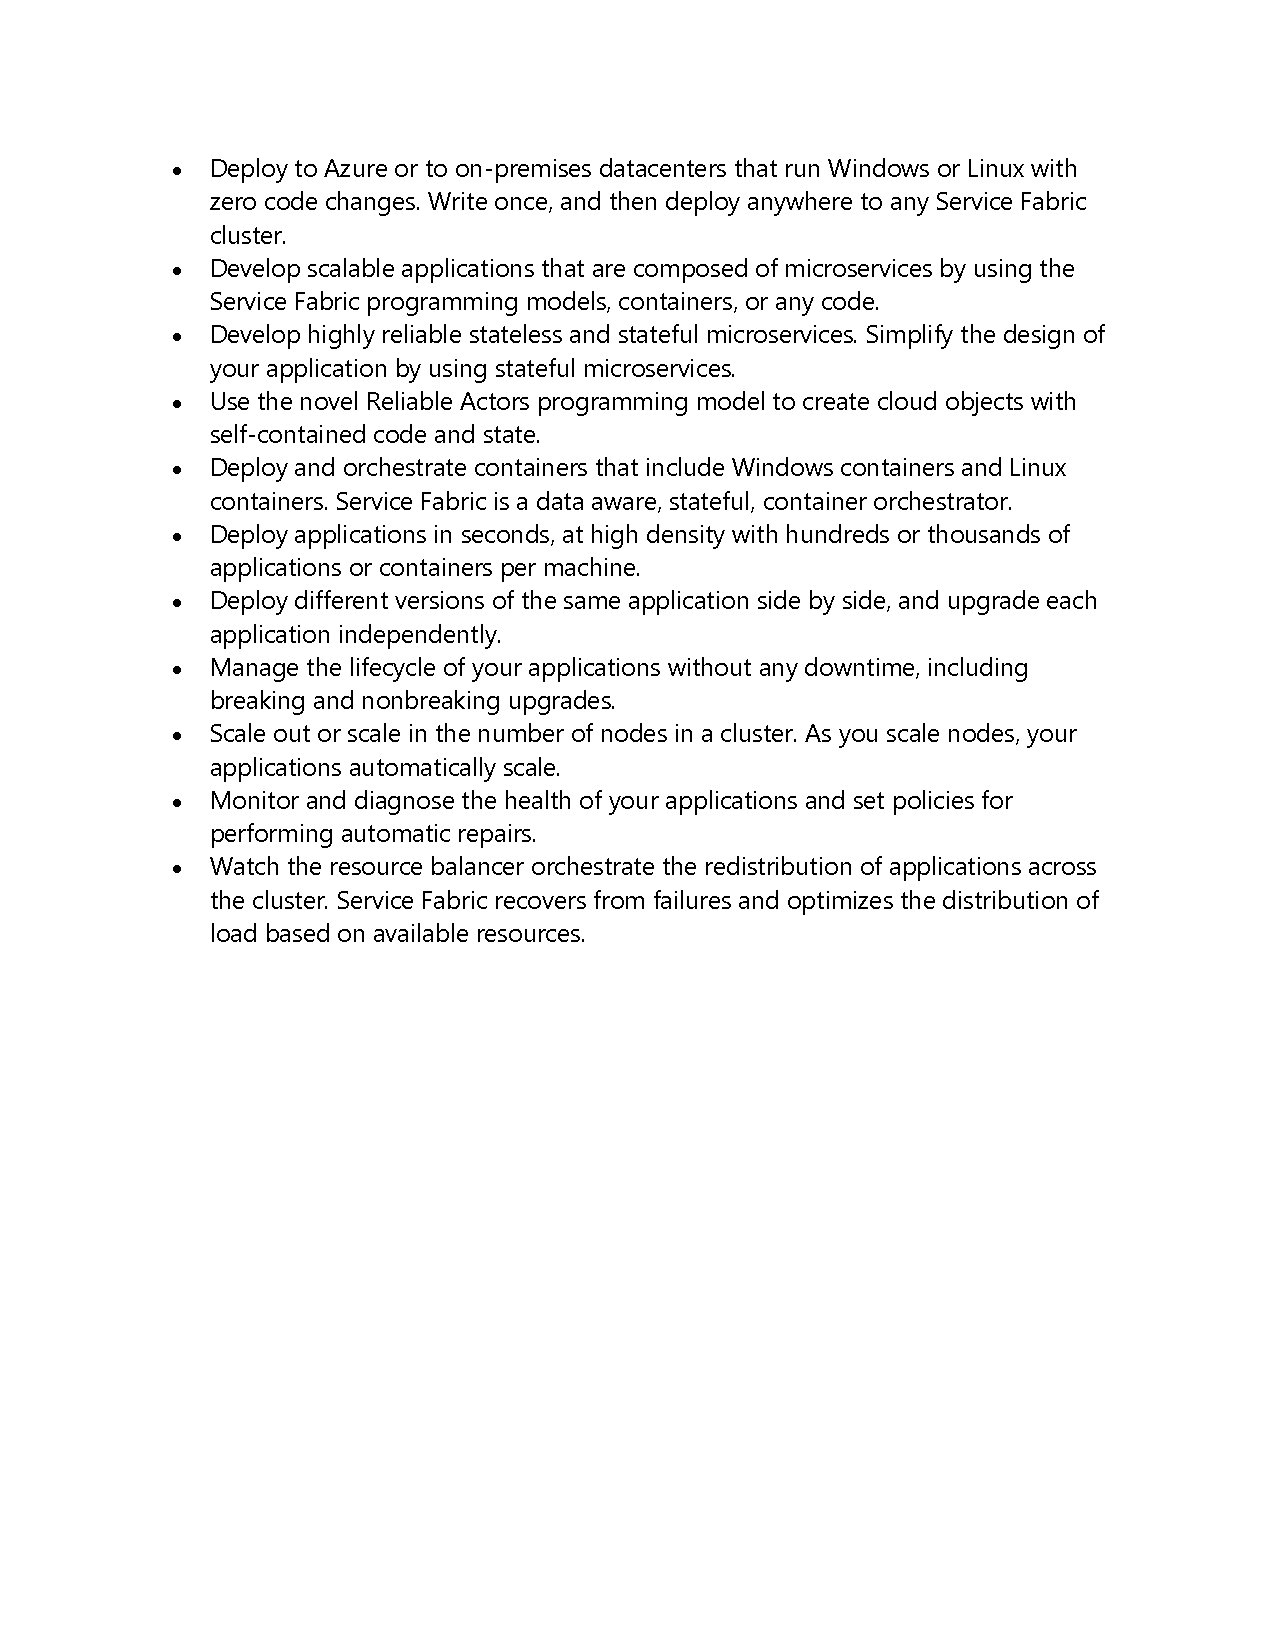
\includegraphics[width=\columnwidth]{images/fig2.pdf}
  \caption{General Resource Manager Function}
\label{f:architecture}
\end{figure*}

Given figure 2, during runtime there are a whole bunch of changes
which could happen. For example, there could be some changes in the
amount of resources services consume, some service failures, or some
nodes join and leave the cluster. All the changes on a specific node
are aggregated and periodically sent to the central Resource Manager
service (1,2) where they are aggregated again, analyzed, and stored.
Every few seconds that central service looks at all the changes and
determines if there are any actions necessary (3). For example, it
could notice that nodes have been added to the cluster and are empty
and decide to move some services to those nodes. It could also notice
that a node is overloaded, or that certain services have failed (or
been deleted), freeing up resources on other nodes.

Figure 3 shows how the Resource Manager reacts to the scenario we
painted earlier.

\begin{figure*}[!ht]
  \centering
\includegraphics[width=\columnwidth]{images/fig3.pdf}
  \caption{Resource Manager Reconfigures the Cluster}
\label{f:architecture}
\end{figure*}

As soon as the Resource Manager determines that changes are necessary
it coordinates with other system services (in particular the Failover
Manager) to make the necessary changes. Then the change requests are
sent to the appropriate nodes (4). In this case, we presume that the
Resource Manager noticed that Node 5 was overloaded, and so decided to
move service B from N5 to N4. At the end of the reconfiguration (5),
the cluster looks like this what we have in figure 3

\section{Resource Management Mechanism}

\subsection{Fault Domains}
In a distributed architecture such as aim a microservice a fault
domain is any area of coordinated failure. A single machine is a fault
domain since it can die for various reasons, for example from power
supply failures or drive failures. Furthermore, a collection of
machines connected to the same Ethernet switch are in the same fault
domain, as would be those connected to a sole source of power.

In setting up a cluster, a lot of attention is required for the
possible areas of failure. The fault domains should therefore be set
up so that Service Fabric can automatically and smartly determine or
triage where or how to place the services in the cluster in case of a
failure.

\subsection{Upgrade Domains}
Upgrade Domains are another feature that helps the Service Fabric
Resource Manager to understand the layout of the cluster so that it
can plan ahead for failures. Upgrade Domains define areas (sets of
nodes, really) that will go down at the same time during an upgrade.

Upgrade Domains are a lot like Fault Domains, but with a couple key
differences. First, Upgrade Domains are usually defined by policy;
whereas Fault Domains are rigorously defined by the areas of
coordinated failures (and hence usually the hardware layout of the
environment). Another difference is that Upgrade Domains are not
hierarchical – they are more like a simple tag than a hierarchy.

There are pros and cons to having large numbers of upgrade domains –
the pro is that each step of the upgrade is more granular and
therefore affects a smaller number of nodes or services. This results
in fewer services having to move at a time, introducing less churn
into the system and overall improving reliability (since less of the
service will be impacted by any issue). The downside of having many
upgrade domains is that Service Fabric verifies the health of each
Upgrade Domain as it is upgraded and ensures that the Upgrade Domain
is healthy before moving on to the next Upgrade Domain. The goal of
this check is to ensure that services have a chance to stabilize and
that their health is validated before the upgrade proceeds, so that
any issues are detected. The tradeoff is acceptable because it
prevents bad changes from affecting too much of the service at a time.

Too few upgrade domains have their own side effects – while each
individual upgrade domain is down and being upgraded a large portion
of your overall capacity is unavailable. For example, if there are
only three upgrade domains then a third of the overall service or
cluster capacity is down at a time. There’s no real limit to the total
number of fault or upgrade domains in an environment, or constraints
on how they overlap. Common structures that are 1:1 ratio (where each
unique fault domain maps to its own upgrade domain as well) an Upgrade
Domain per Node (physical or virtual OS instance), and a “striped” or
“matrix” model where the Fault Domains and Upgrade Domains form a
matrix with machines usually running down the diagonal.

Defining Fault Domains and Upgrade Domains is done automatically in
Azure hosted Service Fabric deployments; Service Fabric just picks up
the environment information from Azure. In turn the Service Fabric
admin can pick the number of required domains. In Azure both the fault
and upgrade domain information look like a “single level” view, but it
really is encapsulating information from lower layers of the Azure
stack and just presenting the logical fault and upgrade domains from
the user’s perspective.

A point of note though. If the cluster is being set up manually, (or
just want to try running a particular topology on the development
machine) then the fault domain and upgrade information has to be
explicitly provided.

\subsection{Capacity Management}
One of the most important jobs of any orchestrator is to help manage
resource consumption in the cluster. Resource optimization ensures
that no nodes are hot (leading to resource contention and poor
performance) nor cold (wasted resources). Other important function is
also to ensure that the nodes don’t run out of resources.

To ensure nodes don’t run out of resources, Service Fabric represents
resources as things called “Metrics”. Metrics are the units by which
any logical or physical resource is described or exposed to Service
Fabric. Examples of metrics are things like “WorkQueueDepth” or
“MemoryInMb”. Metrics are different from constraints and node
properties in that node properties are generally static descriptors of
the nodes themselves, whereas metrics are about physical resources
that services consume when they are running on a node. So a property
would be something like HasSSD and could be set to true or false, but
the amount of space available on that SSD (and consumed by services)
would be a metric like “DriveSpaceInMb”. Capacity on the node would
set the “DriveSpaceInMb” to the amount of total non-reserved space on
the drive, and services would report how much of the metric they used
during runtime.

If all resource balancing are turned off, Service Fabric’s Resource
Manager would still be able to ensure that no node ended up over its
capacity (unless the cluster as a whole was too full). Capacities are
the mechanism that Service Fabric uses to understand how much of a
resource a node has, from which we subtract consumption by different
services (more on that later) in order to know how much is left. Both
the capacity and the consumption at the service level are expressed in
terms of metrics.

During runtime, the Resource Manager tracks how much of each resource
is present on each node (defined by its capacity) and how much is
remaining (by subtracting any declared usage from each service). With
this information, the Service Fabric Resource Manager can figure out
where to place or move replicas so that nodes don’t go over capacity.

It is also possible that a service’s load changes dynamically. In this
case it’s possible that where a replica or instance is currently
placed becomes invalid since the combined usage of all of the replicas
and instances on that node exceeds that node’s capacity. In this case,
Service Fabric resource management automatically kicks in and gets the
node back below capacity by moving one or more of the replicas or
instances on that node to different nodes. When doing this the
Resource Manager tries to minimize the cost of all the movements.

\subsection{Cluster Capacity}
A good question is how does Service Fabric keep the overall cluster
from being too full? To achieve this, there are some controls that are
baked in to prevent basic errors. The first is to prevent the creation
of new workloads that would cause the cluster to become full.

For instance, if we were to create a simple stateless service and it
has some load associated with it. For this service, let’s say that it
cares about some resource (let’s say DiskSpace) and that by default it
is going to consume 5 units of DiskSpace for every instance of the
service and we’ll like to create 3 instances of the service. That
means we need 15 units of DiskSpace to be present in the cluster in
order to create these service instances. Service Fabric will
continually calculate the overall capacity and consumption of each
metric, so that it can easily make the determination and reject the
create service call if there’s insufficient space.

Note that since the requirement is only that there be 15 units
available, this space could be allocated in different ways; it could
be one remaining unit of capacity on 15 different nodes, for example,
or three remaining units of capacity on 5 different nodes, etc. If
there isn’t sufficient capacity on three different nodes, Service
Fabric will reorganize the services already in the cluster in order to
make room on the three necessary nodes. Such rearrangement is almost
always possible unless the whole cluster is almost entirely full,
however it can take some time to complete, potentially delaying the
start of the service instances.

To further manage cluster capacity, Service Fabric also allows adding
some reserved buffer to the capacity specified at each node. This
setting is optional, but it allows people the reservation of some
portion of the overall node capacity so that it is only used to place
services during upgrades and failures – cases where the capacity of
the cluster is otherwise reduced. In the current architecture, buffer
is specified globally per metric for all nodes via the
ClusterManifest. The value picked for the reserved capacity will be a
function of which resources the services are more constrained on, as
well as the number of fault and upgrade domains in the
cluster. Generally, more fault and upgrade domains means that a lower
number of buffered capacity can be picked, since a smaller amount of
your cluster is to be unavailable during upgrades and failures.

\subsection{Placement Policies}
There are many different additional rules that are important
especially if a Service Fabric cluster is spanned across a geographic
distance, for example in multiple datacenters or Azure regions, or if the
environment spans multiple areas of geopolitical control. Most of these
could be configured via node properties and placement constraints
mentioned earlier. However, some are more complicated. In any case,
just like placement constraints, placement policies can be configured
on a per-service basis as described below.

\begin{verbatim}
- InvalidDomain – This allows specifying that a particular
  Fault Domain is invalid for a specific workload.
  This is useful in ensuring that a particular service
  never runs in a particular area,
  for example for geopolitical or corporate policy reasons.
 
- PreferPrimaryDomain – Preferred Primary domain control
  allows the selection of the fault domain in which
  the primary should exist if it is possible to do so. 
  When everything is healthy the primary will
  end up in this domain. Should the domain or the
  primary replica fail or be shut down for some reason
  the Primary will be migrated to some
  other location. When possible, it will move back
  to the preferred domain.

- RequireDomainDistribution – Require domain distribution
  is another option which can be used to prevent
  some situations. Notice that in
  the above example it is possible that temporarily
  multiple replicas
  are packed into the same datacenter. In this case, the
  RequireDomainDistribution flag ensures that the 
  replicas are always
  in separate domains. This means that temporarily
  the cluster is running at below the target number
  of replicas until nodes in a viable domain come back. 
  For small numbers of replicas this could
  result in quorum loss. Since most clusters run
  with more than 3
  replicas, the default is to not require domain
  distribution and let
  balancing and failover handle cases normally even
  if that means that temporarily a domain has multiple
  replicas packed into it.
\end{verbatim}

Multiple Invalid or Required domains can be configured on a single
service, however the other two (preferred domains and domain
distribution) are only configurable once per service.

\subsubsection{Throttles}
Sometimes, even if the resource manager is configured correctly, the
cluster can get disrupted. The Resource Manager will try its best to fix
everything, but in times like a backstop so that the cluster itself
has a chance to stabilize (the nodes which are going to come back come
back, the network conditions health themselves, corrected bits get
deployed) might have to be considered. To help with these sorts of
situations, the Resource Manager does include several throttles. Note
that these are fairly “big hammers” and generally shouldn’t be used
unless there’s been some careful math done around the amount of
parallel work that can actually be done in the cluster, as well as a
frequent need to respond to these sorts of unplanned macroscopic
reconfiguration events.  By default, the Resource Manager includes the
following default throttles:

\begin{verbatim}
- GlobalMovementThrottleThreshold – this controls the
  total number of movements in the cluster over some time
  (defined as the
  GlobalMovementThrottleCountingInterval, value in seconds)

- MovementPerPartitionThrottleThreshold – this controls
  the total
  number of movements for any service partition 
  over some time (the
  MovementPerPartitionThrottleCountingInterval, 
  value in seconds).
\end{verbatim}

\subsubsection{Defragmentation}
In the previous examples, we’ve discussed balancing in terms of
distributing the load – making sure that all of the nodes are equally
utilized. This is the safest and smartest architecture in terms of
surviving failures since it makes sure that any given failure doesn’t
take out the majority of the workload. The Service Fabric Resource
Manager does support a different strategy as well, which is
defragmentation. Defragmentation generally means that instead of
trying to distribute the utilization of a metric across the cluster,
the system should be architected to consolidate utilization.

Why defragmentation? In the case the load in a cluster is spread out
evenly among the nodes in the cluster, then by implication some of the
resources the node has to offer are used up. This isn’t normally a
problem, but sometimes some workloads create services which are
exceptionally large and consume the majority of a node – say 75
percent - 95percent of a node’s resources would end up dedicated to a
single service. This is actually not a problem as the Resource Manager
will detect on creation that it needs to reorganize the cluster in
order to make room for this large workload and set about making it
happen, but in the meantime that workload has to wait.

Just like file creation or access could get slowed down if a
computer’s hard disk was fragmented and could be sped up by
defragmenting the drive, defragmentation metrics can be configured to
have the Resource Manager proactively try to condense the load of the
services into fewer nodes so that there is (almost) always room for
even large services, enabling them to be created quickly.

In the Resource Manager configuration, the defragmented and normal
metrics can be mixed in the same cluster and the Resource Manager will
do it’s best to consolidate the layout to allow as much of the
defragmentation metrics as it can while trying to spread out the
rest. The results in this case will depend on the number of balancing
metrics compared to the number of defragmentation metrics and their
weights.


\section{Conclusion}
In practice, the Service Fabric Resource Manager is an incredibly
powerful tool for orchestrating microservices.

Increasingly, winning enterprise operating models require agility and
scalability across regulatory, compliance and business constraints on
global scale and at a much more frequent pace than we’ve ever
witnessed. The implication of this is that the underlying technology
architecture that supports a business must also be equally adaptable
to the rapid changes required of the operating models.

Microservices architecture enables the business to run multiple
loosely coupled but related services on the enterprise technology
stack. The rapid changes required of businesses and the
‘loosely-coupled’ nature of microservice then requires a carefully
managed orchestration.

Azure Service Fabric is a Microsoft microservices technology offering
that enables enterprises meet the business objectives outlined
above. The Service Fabric Resource Manager enables enterprises to
exercise tight control and orchestrate resources in their Service
Fabric-based microservices. The Resource Manager enforces policies,
improve utilization, and get carbon-based life forms out of the
critical path when reacting to failures, managing processes like
upgrades, and trying to game out capacity and load scenarios in the
Service Fabric cluster.


\begin{acks}

  The authors would like to thank Dr.~Gregor~von~Laszewski for his
  support and suggestions to write this paper.

\end{acks}

\bibliographystyle{ACM-Reference-Format}
\bibliography{report}
